\section{Background}

% ------------------- Introduce Bayes --------------------------

\subsection{Bayesian Statistics}

This paper does not aim to serve as a guide to Bayesian statistics, nor an
explicit introduction to the theory. Nonetheless, some background knowledge is
necessary in understanding the theory and assumptions motivated throughout the
paper.

In Bayesian statistics, the foundational interpretation of probability differs
from traditional frequentist statistics. In the more familiar frequentist approach,
probability is defined as the long-run frequency of an event occurring, the
intuition of which can be built with the example of a coin flip. The
probability of a coin landing on heads is assumed to be a fixed but unknown
quantity, and when a coin is flipped 100 times, and 60 of those flips result in
heads, the probability of heads is defined as 0.6. 

In contrast, Bayesian statistics defines probability as a measure of belief and
model parameters - like the true fairness of a coin - are assumed to be random
variables. Our belief about the probability of heads is represented by a prior
distribution, which is updated based on observed data. If a coin is flipped 100
times and heads observed 60 times, this prior belief about the probability of
heads is updated to a posterior distribution that reflects our new
understanding of the coin's behavior, taking into account both the observed
data and our initial belief. This posterior distribution allows us to quantify
our uncertainty about the probability of heads and make predictions - or
inferences - about future coin flips.

\subsubsection{Bayes' Theorem}

The framework for updating beliefs in Bayesian statistics is Bayes' Theorem;
derived from the definition of conditional probability. Bayes' Theorem
describes the probability of an event, based on prior knowledge of conditions 
that might be related to the event, and observed evidence. 
The general form of Bayes' Theorem is given by:
\begin{equation}
  P(A|B) = \frac{P(B|A)P(A)}{P(B)}
\end{equation}
Applications of the Bayesian framework are vast; the belief in any hypothesis can
be logically updated when new evidence is encountered.
\begin{equation}
  P(\text{Hypothesis}|\text{Evidence}) = \frac{P(\text{Evidence}|\text{Hypothesis})P(\text{Hypothesis})}{P(\text{Evidence})}
\end{equation}
In the context of Bayesian modeling, we are interested in updating our beliefs
about the parameters of a model given some observed data.
\begin{equation}
  P(\text{Parameters}|\text{Data}) = \frac{P(\text{Data}|\text{Parameters})P(\text{Parameters})}{P(\text{Data})}
\end{equation}
\begin{table}[h]
\centering
\begin{tabular}{lll}
\toprule
Term & Symbol & Description \\
\midrule
Posterior & $P(\text{Parameters}|\text{Data})$ & Updated belief about the parameters given the data \\
Likelihood & $P(\text{Data}|\text{Parameters})$ & Probability of observing the data given the parameters \\
Prior & $P(\text{Parameters})$ & Initial belief about the parameters before observing the data \\
Evidence & $P(\text{Data})$ & Probability of observing the data \\
\bottomrule
\end{tabular}
\caption{Components of Bayes' theorem in the context of Bayesian modeling.}
\label{tab:bayes_theorem}
\end{table}

\subsubsection{Priors}
Unique to Bayesian statistics is the concept of prior distributions. Priors are
probability distributions that represent the beliefs about the model parameters
before observing any data. \cite{clinical} does a fine job of illustrating the
impact of priors on the posterior distribution, shown in figure
\ref{fig:prior-impact}. 
\begin{figure}
  \begin{center}
    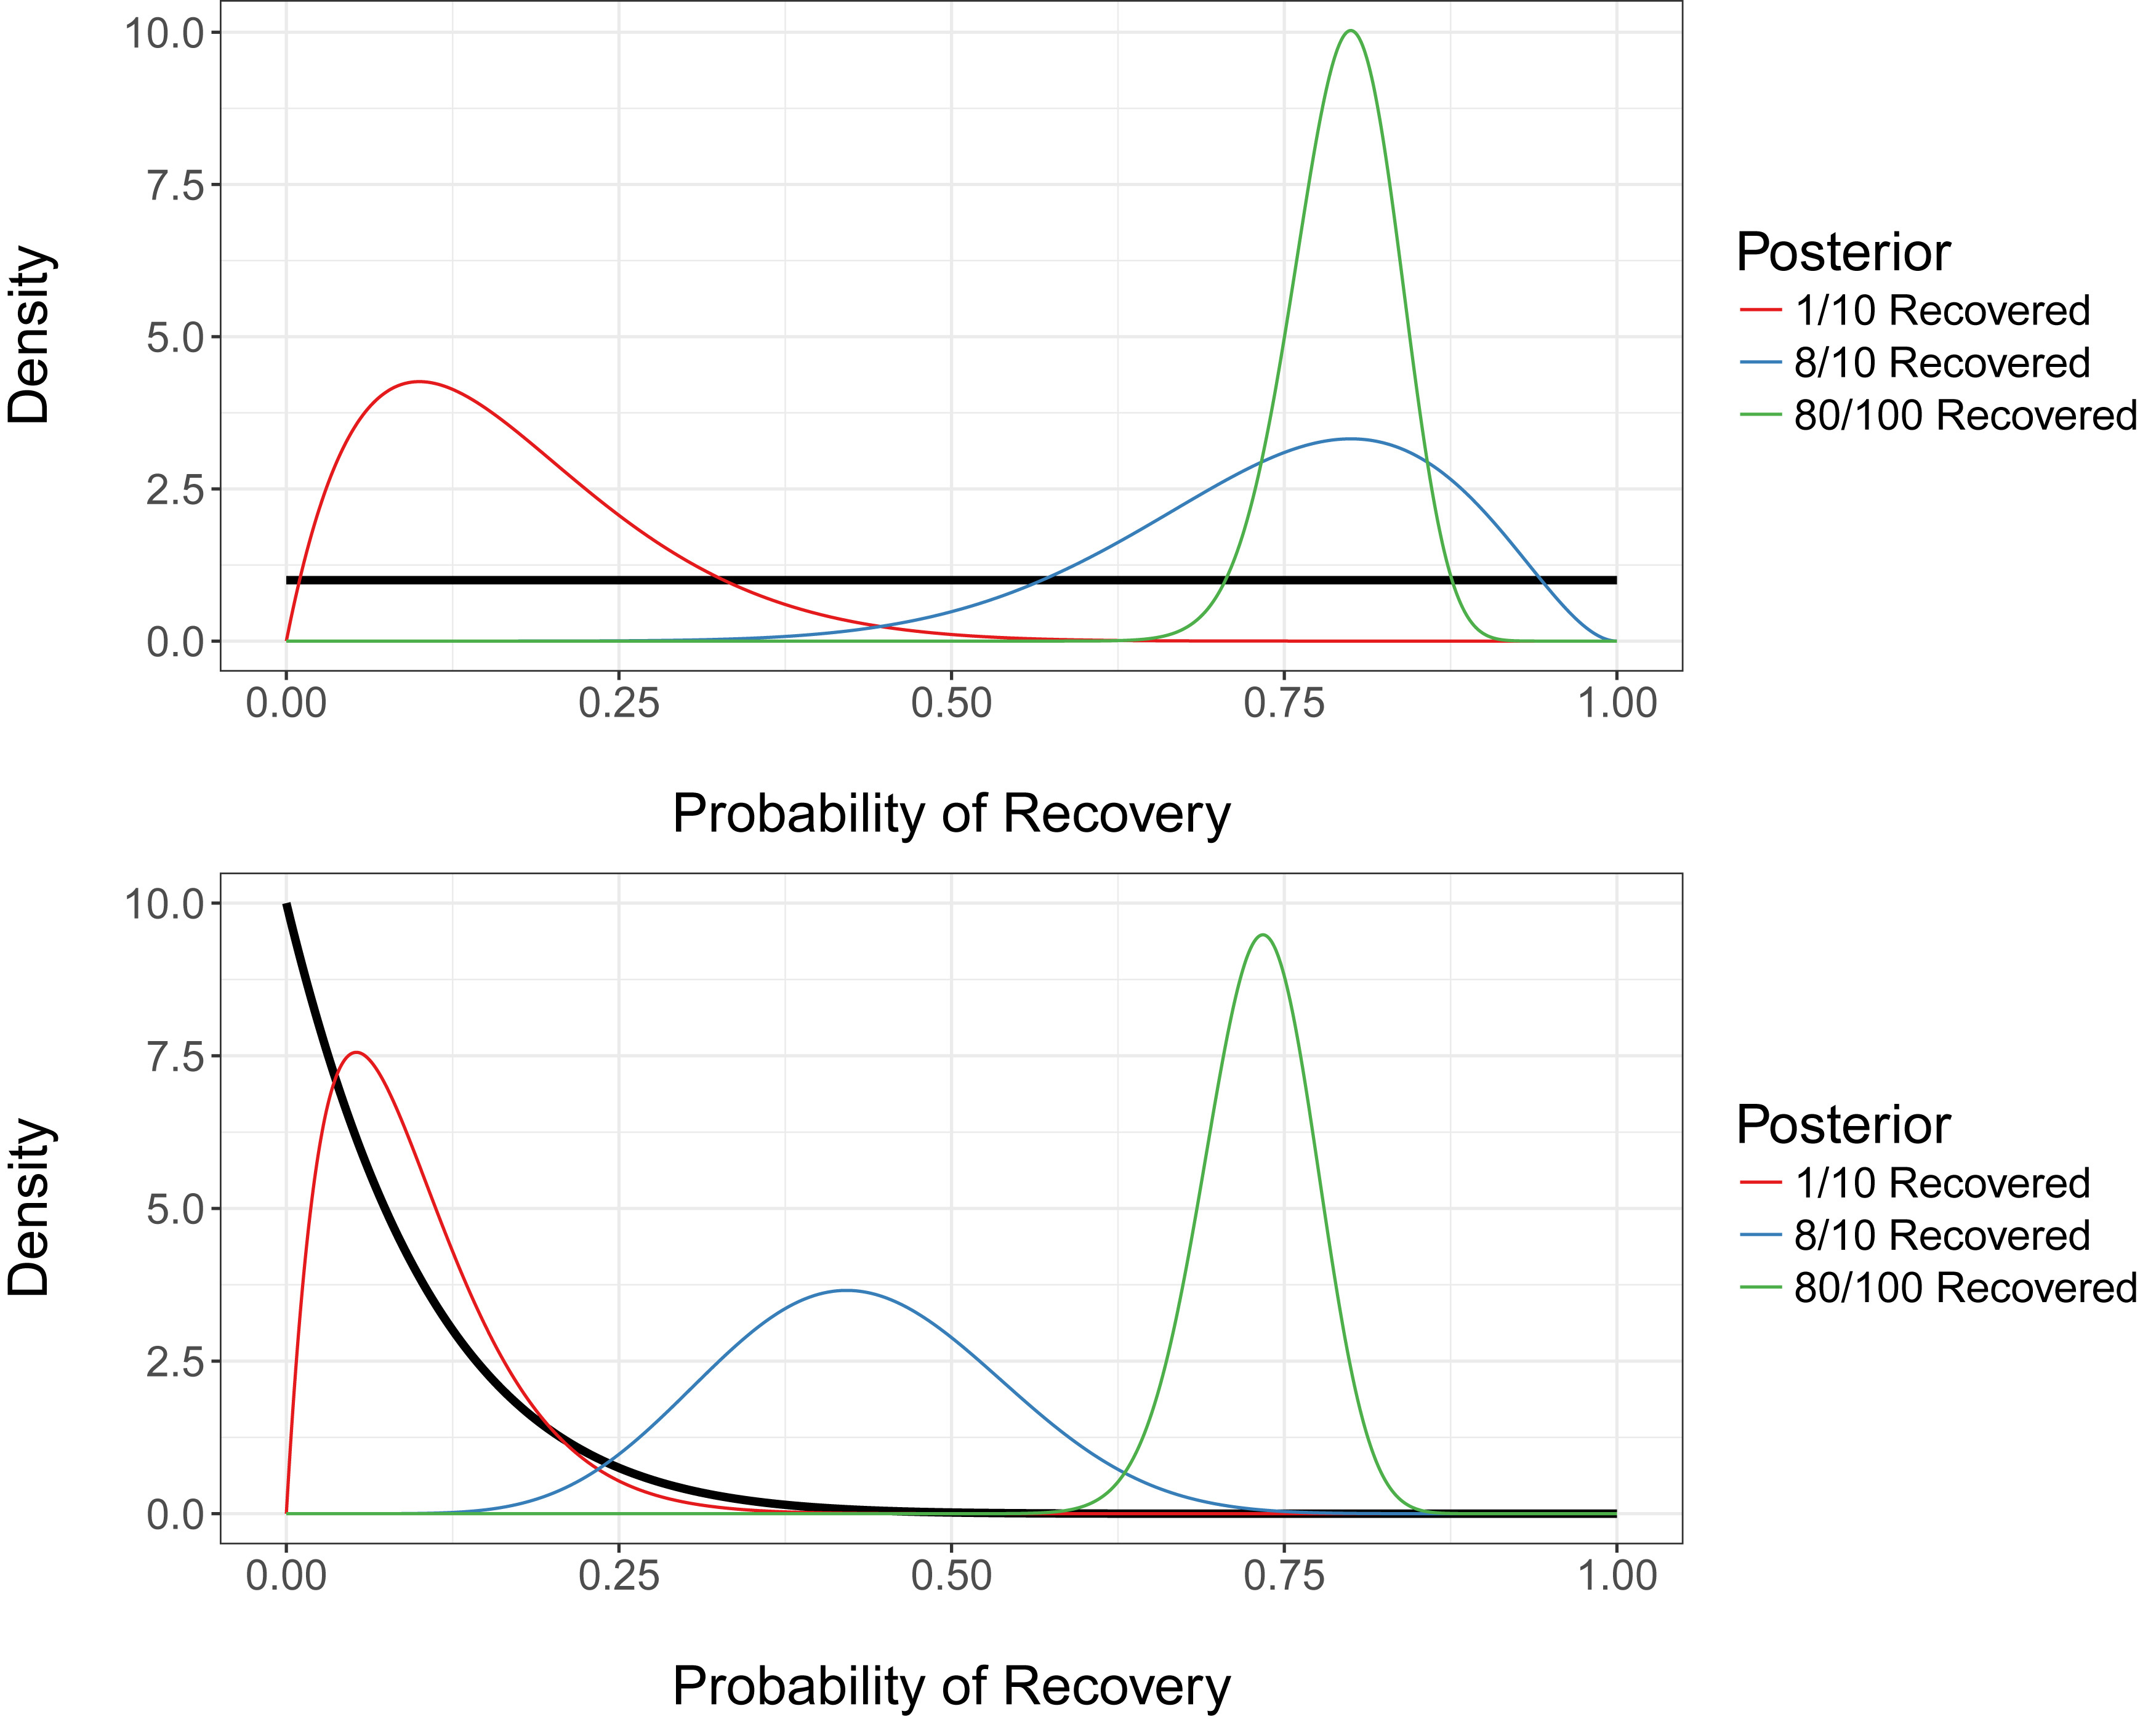
\includegraphics[width=0.5\textwidth]{../imgs/prior-impact.jpg}
  \end{center}
  \caption{Plots demonstrating the impact of different priors and data on posterior distributions. The top figure is for a flat prior distribution and the bottom figure is for an informative prior distribution. Solid black line is the prior distribution, colored lines are the posterior distributions, \cite{clinical}.}
  \label{fig:prior-impact}
\end{figure}
They are often a talking point in the validity of experiments utilising a
Bayesian approach as, while incorporation of prior knowledge can be a key
factor in Bayesian models outperforming other frequentist models, especially
when the amount of data is limited; they can also be seen as a daunting source
of subjectivity.
There are two main philosophies when it comes to selecting priors, objective
and subjective Bayesianism. 

\textbf{Objective Bayesianism} aims to minimise the influence of personal
beliefs on the analysis by using priors that are as non-informative as
possible. Objective priors, often called non-informative or reference priors,
are chosen based on the principle of indifference or maximum entropy, which
tries to represent a state of ignorance about the parameters. The goal is to
allow the data to have the most influence on the posterior distribution. This
approach is often favored when there is limited prior knowledge or when
researchers wish to avoid potential bias from subjective beliefs. However, even
with the best intentions in mind, no prior can be truly non-informative, and
objective priors can still carry some level of subjectivity in their selection.

\textbf{Subjective Bayesianism}, on the other hand, embraces the idea that
personal beliefs and prior knowledge should be incorporated into the analysis.
Subjective priors are chosen based on a researcher's knowledge, expertise, and
beliefs about the parameters of interest. This approach allows for the
integration of existing information and expert opinions, which can result in
more accurate and informative inferences, especially in cases where data are
limited or noisy. Some argue that subjective priors can introduce bias, as they
rely on the researcher's personal beliefs. However, the opposing argument that
scientific research inherently subjective to some degree, and transparency
about the choice of priors, at worst allows for open evaluation and discussion
within the research community.
\cite{clinical} addresses the viewpoint that, on the surface, it might seem
outright wrong that two otherwise identical experiments can yield different
results, simply because different prior beliefs were defined. Baldwin and
Larson show that this argument is mitigated by the fact that subjectivity is
inherent in research, researchers' background knowledge informs prior choices,
all statistical methods involve assumptions, and data likelihood choices often
have greater impact than priors. They claim it is justifiable from a scientific
standpoint to integrate prior knowledge about parameters into the models. That
being said, priors should always be selected with care and their impacts
transparently communicated. 

Both philosophies are worth considering when selecting priors, and while this
paper is grounded more in the objective approach, the subjective approach is
also considered.

\subsubsection{Markov Chain Monte Carlo}

Given Bayes' Theorem defines the closed form solution of the posterior
distribution; a natural question to ask is why and where is sampling necessary?
The short answer is that, in most cases, it is not possible to analytically
compute the posterior distribution, due to the intractability of the evidence
term. Computing the evidence term, or marginal likelihood, $P(D)$,
involves integrating over all possible values of the parameters, which is often
computationally infeasible \cite{mcmc}.

Markov Chain Monte Carlo (MCMC) is the name for a class of algorithms whose
goal is to draw samples from a distribution, without needing to know the
specific probability density at any point. It is enough to realise that, as per
Bayes' theorem, the posterior distribution of the model parameters is
proportional to the product of the likelihood and the prior, up to a
normalising constant. From a high level, MCMC achieves this with stochastic
exploration of the parameter space, guided by the likelihood function which
reveals regions of higher posterior probability. The likelihood function answers the
question: given this sampled instance of the parameters, how likely is it that
the observed data would have been generated by the model? Areas in the
parameter space with higher probability are then explored - or sampled from -
more frequently, and the result is a set of samples that have been drawn from a
distribution proportional to the posterior distribution. With enough samples,
the posterior can be approximated by the distribution of the samples.
Further reading on MCMC can be found in \cite{mcmc}, as well as alternative
methods for approximating the posterior distribution, such as Variational
Inference \cite{vi}, but deeper understanding of these methods is not required
for this paper.

In this study, the MCMC algorithm employed is the No-U-Turn Sampler (NUTS)
\cite{nuts}, an extension of the Hamiltonian Monte Carlo (HMC) algorithm
\cite{hmc}. NUTS is the default sampler in the PyMC library \cite{pymc} and
requires less configuration than HMC, while still being able to approximate
complicated posterior distributions efficiently.

\textbf{Assessing Convergence}

The fitting of a model, $M$, on data, $D$, refers to the characterisation of
the posterior distribution of a model's parameters, $\theta$, given the data,
$D$, \cite{pymc-modelling}.
\begin{equation}
  \label{eq:posterior}
  p(\theta|D,M) = \frac{p(D|\theta,M)p(\theta|M)}{p(D|M)}
\end{equation}

We know that, as the number of samples increases, the MCMC distribution
converges to the stationary distribution, but there is no universal threshold
for the number of samples required to reach convergence, so assessing
convergence is an important step in the fitting process. In \texttt{PyMC},
models are fit using the \texttt{sample} function; this is where various
parameters of the MCMC sampling algorithm are specified. Among others, these
include:
\begin{itemize}
  \item \texttt{draws} - the number of samples to draw from the posterior
  \item \texttt{tune} - the number of samples to discard as burn-in \cite{burn-in}
  \item \texttt{chains} - the number of independent chains to run
  \item \texttt{target\_accept} - the target acceptance probability for the sampler
\end{itemize}
PyMC provides a number of built-in convergence diagnostics, which were all used
in combination with visual inspection of trace plots, Figure
\ref{fig:trace-plots}, to assess convergence. These include:
\begin{itemize}
  \item Monte Carlo Standard Error of the Mean
  \item Monte Carlo Standard Error of the Standard Deviation
  \item Effective Sample Size for the Bulk
  \item Effective Sample Size for the Tail
  \item Gelman-Rubin Diagnostic
\end{itemize}
The value of the Gelman-Rubin diagnostic (R-Hat) provides evidence that the multiple chains
converged to the same posterior distribution by measuring the ratio of between-chain variance to 
within-chain variance. Values close to 1 indicate convergence, values greater than 1.1 are 
considered to demonstrate non-convergence \cite{statrethinking}.

Effective sample size (ESS) is a measure of the number of independent samples 
that would be required to achieve the same precision as the MCMC samples.
The ESS for the bulk is the ESS for the samples excluding the first 50\% of the samples, 
and the ESS for the tail is the ESS for the samples excluding the first 10\% of the samples 
\cite{statrethinking}. Ideally, the ESS should be close to the number of samples drawn, 


\subsubsection{Trace plots}

Trace plots are a useful tool for visualising the MCMC sampling process. They 
show the value of each parameter over the course of the sampling process, 
allowing for manual convergence assessment and identification of potential problems with
the sampling process. Figure \ref{fig:trace-plots} shows the trace plots for 
the parameters of the model fit to the data.
A simple and widely-used approach to evaluate convergence is by examining trace plots. A trace plot is a line graph where the x-axis represents the iteration, and the y-axis shows the sampled parameter value. Trace plots, such as those generated by the brms package for , , and $\sigma$, should exhibit two key characteristics: stationarity and good mixing (McElreath, 2016, p. 253). Stationarity implies that the samples remain within the posterior distribution and accurately represent it (Kruschke, 2015). In other words, the trace plot should not deviate outside the posterior distribution but maintain its position within the same parameter space throughout iterations and chains. Good mixing signifies that consecutive samples within a chain should not be correlated. Instead, the trace plot should oscillate within the posterior, moving both upwards and downwards, indicating that the chain is collecting samples from all areas of the posterior or thoroughly exploring the posterior distribution. The trace plots in Fig. 3 exhibit both stationarity and good mixing (refer to McElreath, 2016, pp. 258 and 262 for examples of problematic trace plots).

\subsubsection{Autocorrelation} 
Autocorrelation is a statistical measure that quantifies the similarity between
observations of a series conditioned on a specific time lag. The concept
has been mentioned in the context of MCMC sampling, but is arguably more
traditionally assocated with time dependent data, such as the present case
study; and while the concept remains the same, it is important to understand the 
implications of autocorrelation in both contexts. 

\textbf{Autocorrelation in MCMC sampling}  refers to the dependence between
samples in the MCMC chain (Robert \& Casella, 2013). Since MCMC methods generate
samples sequentially, it is possible for consecutive samples to be correlated.
High autocorrelation between samples indicates that the MCMC chain is moving
slowly through the parameter space and not exploring the posterior distribution
efficiently (Brooks et al., 2011).

Autocorrelation in MCMC samples is undesirable, as it reduces the effective
sample size, which in turn leads to less precise estimates of the posterior
mean, variance, or other quantities of interest (Gelman et al., 2014). To
assess the autocorrelation in MCMC samples, we calculate the autocorrelation at
different lag times within the chain. If the autocorrelation is high, it
suggests that the MCMC sampling process is not efficient, and we might need to
run the chain for more iterations, use a different MCMC algorithm, or adjust
the tuning parameters to improve the sampling efficiency (Andrieu et al.,
2003).

\textbf{Autocorrelation in time series data} measures the degree of similarity
between a variable's current value and its past values (Brockwell \& Davis,
2002). If a time series has strong autocorrelation, it means that the values of
the series at different time points are highly dependent on each other. This
information is useful for time series forecasting, as it helps to identify
patterns and trends in the data that can be exploited to make more accurate
predictions (Hyndman \& Athanasopoulos, 2018).

For instance, if a time series exhibits high positive autocorrelation at a
specific time lag, it suggests that the values at that time lag are similar to
the current values. Conversely, if the time series exhibits high negative
autocorrelation, it implies that the values at that time lag are dissimilar to
the current values. Knowing the autocorrelation structure of a time series can
be crucial for selecting appropriate forecasting models, such as autoregressive
(AR) models, which use past values as predictors for future values (Hamilton,
1994).

\subsection{Bayesian Model Comparison \& Evaluation}
Bayesian statistics includes its own philosophy of model comparison, parts of
which will be applied to compare and select the best of the various models
later in the study. The Bayesian approach to model comparison aims to identify
the model that achieves the best trade-off between goodness of fit and model
complexity, in order to provide the most accurate and informative explanation
of the observed data.

In his book 'Statistical Rethinking', Richard McElreath (2016) motivates and 
explains techniques for Bayesian model comparison in great detail. For this 
paper, knowledge of the inner workings of the techniques is not required, 
however it helps to understand the intuition behind the techniques foundational 
to the Bayesian approach to model comparison.

\begin{itemize}
  \item \textbf{Bayes Factor} - A measure of the relative evidence of one model
    over another, calculated by taking the ratio of the marginal likelihoods of
    two models asking: Which model is more likely to have generated the
    observed data?
  \item \textbf{WAIC} - Widely Applicable Information Criterion, a measure of
    out-of-sample predictive accuracy, quantifying the trade-off between
    goodness  of fit and model complexity.
  \item \textbf{LOOCV} - Leave-One-Out Cross-Validation, a measure of
    out-of-sample predictive accuracy, iteratively assessing model fit on
    $len(Data) - 1$ folds of data.
\end{itemize}

\subsection{Data volume and performance}
The second research questions asks: What is the optimal data volume for accurate
revenue prediction? This intuition is based on questioning the common
assumption that the more data is available, the more accurate the model will
be. In the real world, there is no guarantee the complicated underlying revenue
generating process will remain constant over time, therefore there exists the
possibility that encorporating data from the distant past will not only not
lead to better predictive power, but by introducing more noise, may lead to
worse predictions. This is an area that has been researched, but lacks a clear
consensus. 
\cite{big-data-hal-varian} highlights the importance of considering data
quality and recency when incorporating historical data in econometric models.
Hal Varian suggests that using too much historical data or data that is not
directly relevant to the problem at hand can sometimes introduce noise and lead
to worse predictions. However when this notion is explored in
\cite{data-volume-weather}, the authors find that more data is categorically
beneficial in improving the accuracy of a trained model. To this end, this
study aims to explore the relationship between data volume and predictive power
in the context of Bayesian revenue modelling and forecasting.

\subsection{Approaches}

The problem of revenue forecasting is not a new one and there exist a number of
different approaches to time-sensitive prediciton, each with their own
subtleties to consider.
% Statistical modelling 
Traditional statistical modelling techniques are widely used to identify trends
and relationships between variables and make predictons and we will discuss how
Bayesian methods can be a flexible extension of some of these methods. 
% Time series models
Working with time dependent data, time series models are a natural choice and
are widely used in industry for problems similar to the one this paper
addresses. Auto-regressive models, Moving Average models and everything in
between are some examples of time series which take a different approach to
modelling temporal data.
% Machine learning methods
Machine learning methods continue to grow in popularity, the applications of
which extend to a myriad of problems, no doubt including this one. The nature
of this problem prioritises interpretability over predictive power, which is
why we will not be comparing the specific implementations of these methods.
Nevertheless, the general principles of machine learning are worth mentioning
and recognising as a potential alternative to the methods discussed in this
paper.
% Bayesian approach: Advantages and challenges
Finally, Bayesian modelling can have a number of benefits in this context, such
as the capacity to account for past knowledge, quantify uncertainty, and
automatically update the model when new data become available. However,
Bayesian methods can be computationally taxing, particularly for large datasets
and intricate models, and they might necessitate a careful examination of prior
distributions and presumptions.

